\documentclass[a4paper]{article}

\usepackage{graphicx}
\usepackage{parskip}
\usepackage{hyperref}

\author{A. Abdulwahed, M. Kaoula, M. Laruina, R. Mancini}
\title{Distributed Key Value Store using RAFT\\Specification document}
\date{\today}

\begin{document}
    \maketitle

    \section{Introduction}

    The goal of the project is to implement a distributed and strongly 
    consistent in-memory key-value store using the RAFT algorithm for consensus.
    The architecture is highly modular, leading to better flexibility and 
    re-usability. With this choice, synchronization and coordination issues are 
    offloaded to the communication between the modules.

    The possible operations on the distributed KV store will be the following:
    \begin{itemize}
        \item \texttt{V get(K key)}: returns the value associated with the key
        \item \texttt{Map<K,V> getAll()}: returns all key-value pairs
        \item \texttt{void set(K key, V value)}: sets the given value to the 
            provided key
        \item \texttt{void delete(K key)}: deletes the item with the given key
        \item \texttt{void deleteAll()}: deletes all the keys
    \end{itemize}

    The core of the RAFT algorithm will be developed using Erlang and will be 
    generic (section \ref{sec:raft-core}). Using this generic RAFT implementation, 
    another Erlang RPC server will be developed which implements the Key-Value 
    store (section \ref{sec:kv-store}) and provides an interface to access the 
    datastore. Another module will make it possible to access the key-value 
    store from Java, using the \emph{Jinterface} package 
    (section \ref{sec:erlang-java}). 
    This exported interface will be used by a web-server which will provide 
    REST APIs for the key-value store and an administration GUI
    (section \ref{sec:web-server}).

    \section{Architecture}

    \begin{figure}[h]
        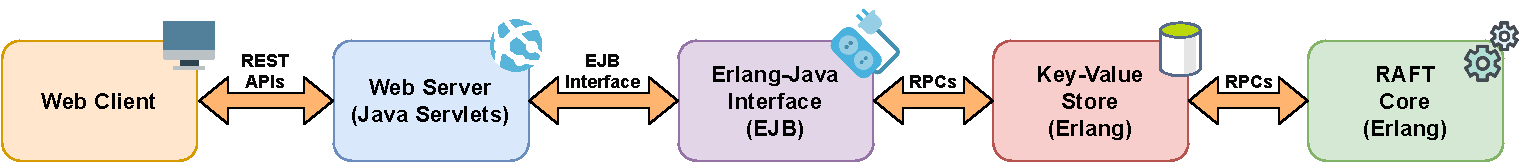
\includegraphics[width=\textwidth]{raft_architecture.pdf}
    \end{figure}

    \subsection{RAFT core}
    \label{sec:raft-core}

    This Erlang module will implement the RAFT finite-state machine (FSM)
    and will take care of all the communication between nodes. Communication
    between nodes needs to be reliable and will be taken care of by the Erlang
    middleware. 

    This module will be implemented using the \emph{gen\_statem} and 
    \emph{gen\_server} Erlang \emph{behaviours}. This module will run on all 
    nodes.

    \subsection{KV store}
    \label{sec:kv-store}

    This Erlang module will implement the Key-Value store. It will need to 
    handle incoming commits from the RAFT core and reply to get and set 
    requests, querying the current master node\footnote{\emph{get} requests can 
    be handled directly by a secondary node if a strong consistency is not 
    required}. All communication with the Erlang core and the \emph{Erlang-Java
    interface} will be done using RPCs.

    This module will be implemented using the \emph{gen\_server} Erlang 
    \emph{behaviour}.
    This module will run on all nodes.

    \subsection{Erlang-Java interface}
    \label{sec:erlang-java}

    This Java module will expose the Erlang KV store to a JEE environment and 
    will be implemented as an EJB. This EJB will provide an interface to 
    view and edit the key-value store and will communicate with the Erlang 
    environment through RPCs using the \emph{Jinterface} package. Communication
    with other EJB will be handled by the JEE runtime.

    \subsection{Web Server}
    \label{sec:web-server}
    This Java module will implement a Web server to server REST APIs and an 
    administrative GUI. It will be implemented using Java Servlets.

\end{document}